\documentclass[a4paper,10pt]{article}
%\documentclass[a4paper,10pt]{scrartcl}

\usepackage[utf8]{inputenc}
\usepackage{graphicx}
\usepackage{float}
\title{Trabajo Práctico 1, Reconocimiento de Patrones}
\author{Federico De Rocco}

\pdfinfo{%
  /Title    (Trabajo Práctico 1, Reconocimiento de Patrones)
  /Author   (Federico De Rocco)
}

\begin{document}
\maketitle
\section{Introducci\'on}
El objetivo de \'este informe es el de descrivir como se resolvi\'o el primer trabajo práctico de la materia Reconocimiento De Patrones. En las siguientes secciones se expondr\'an y explicaran las elecciones que se llevo a cabo para poder lograr \'este objetivo.

\section{Ejercicio 1}
Se nos pide generar una imagen sint\'etica a partir de phantom y despu\'es clasificarla. Se utilizara los mismos valores medios para cada uno de los casos de covarianza. 

\begin{figure}[H]
\centering
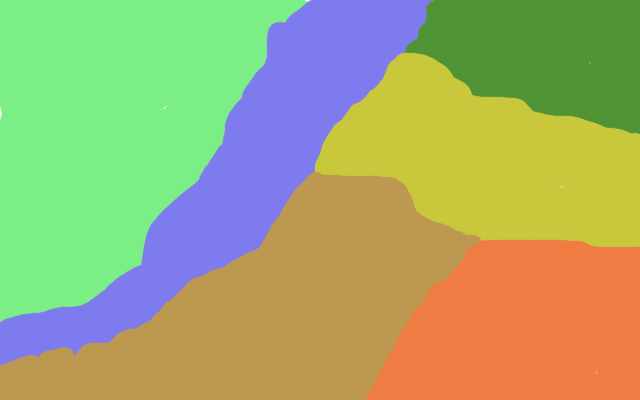
\includegraphics[width=90mm]{phantom.png}
\caption{Imagen original}
\end{figure}

Considerando que tenemos 6 clases distintas utilizaremos lo siguiente:

mus = 
\begin{tabular}{ l c r }
  1 & 2.3 & 1.34 \\
  1.26 & 1.23 & 2.39 \\
  8 & 1.47 & 0.53 \\
  2.01 & 1.99 & 0.60\\
  1.88 & 1.52 & 0.81 \\
  2.39 & 1.24 & 0.67\\
\end{tabular}

\subsection{Utilizando matrices de covarianza isotr\'opicas e iguales entre s\'i}

Se toma las siguientes matrices de covarianza:

sigma1 = 
\begin{tabular}{ l c r }
  0.5 & 0 & 0 \\
  0 & 0.5 & 0 \\
  0 & 0 & 0.5 \\
\end{tabular}


sigma2 =
\begin{tabular}{ l c r }
  20 & 0 & 0 \\
  0 & 20 & 0 \\
  0 & 0 & 20 \\
\end{tabular}


Con estas se generaron las siguientes im\'agenes:

\begin{figure}[H]
\centering
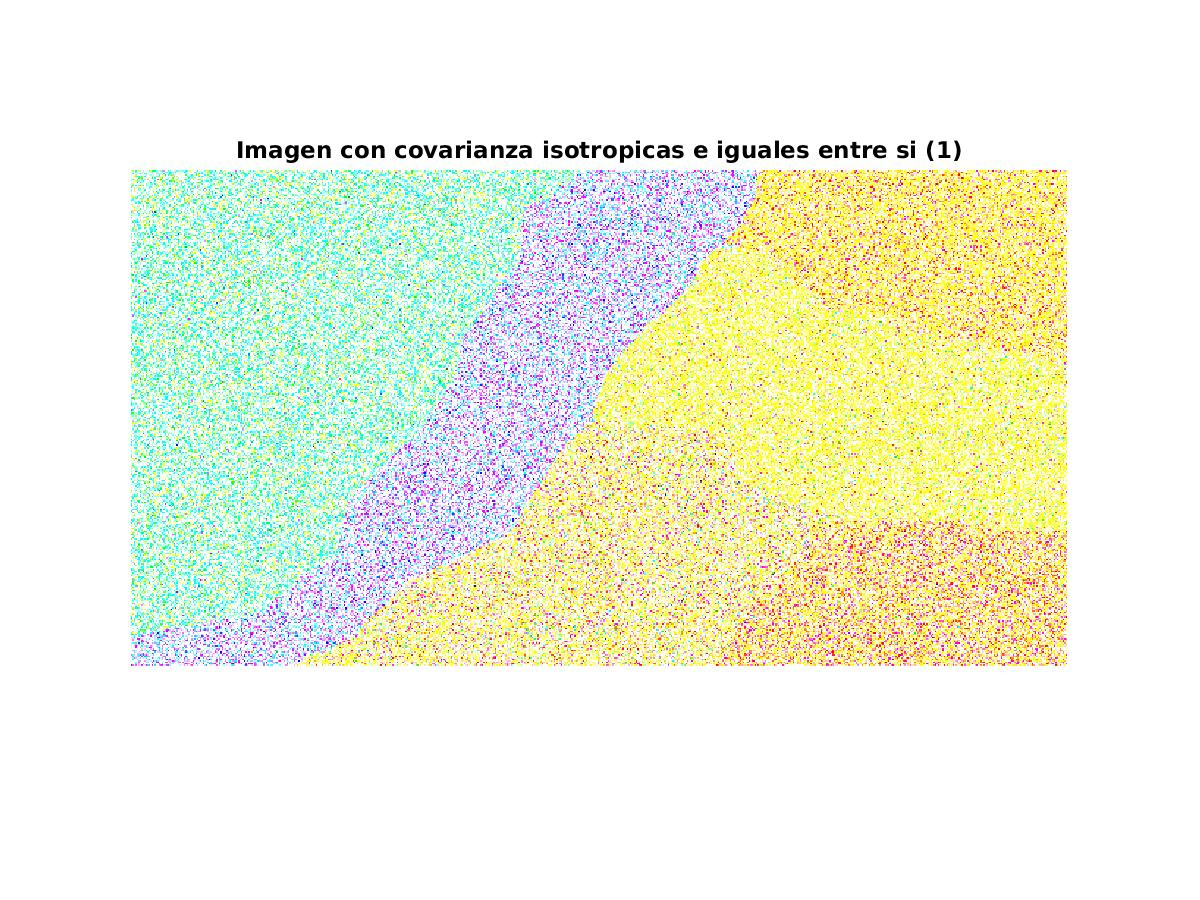
\includegraphics[width=90mm]{imagenII1.jpg}
\caption{Usango sigma1}
\end{figure}


\begin{figure}[H]
\centering
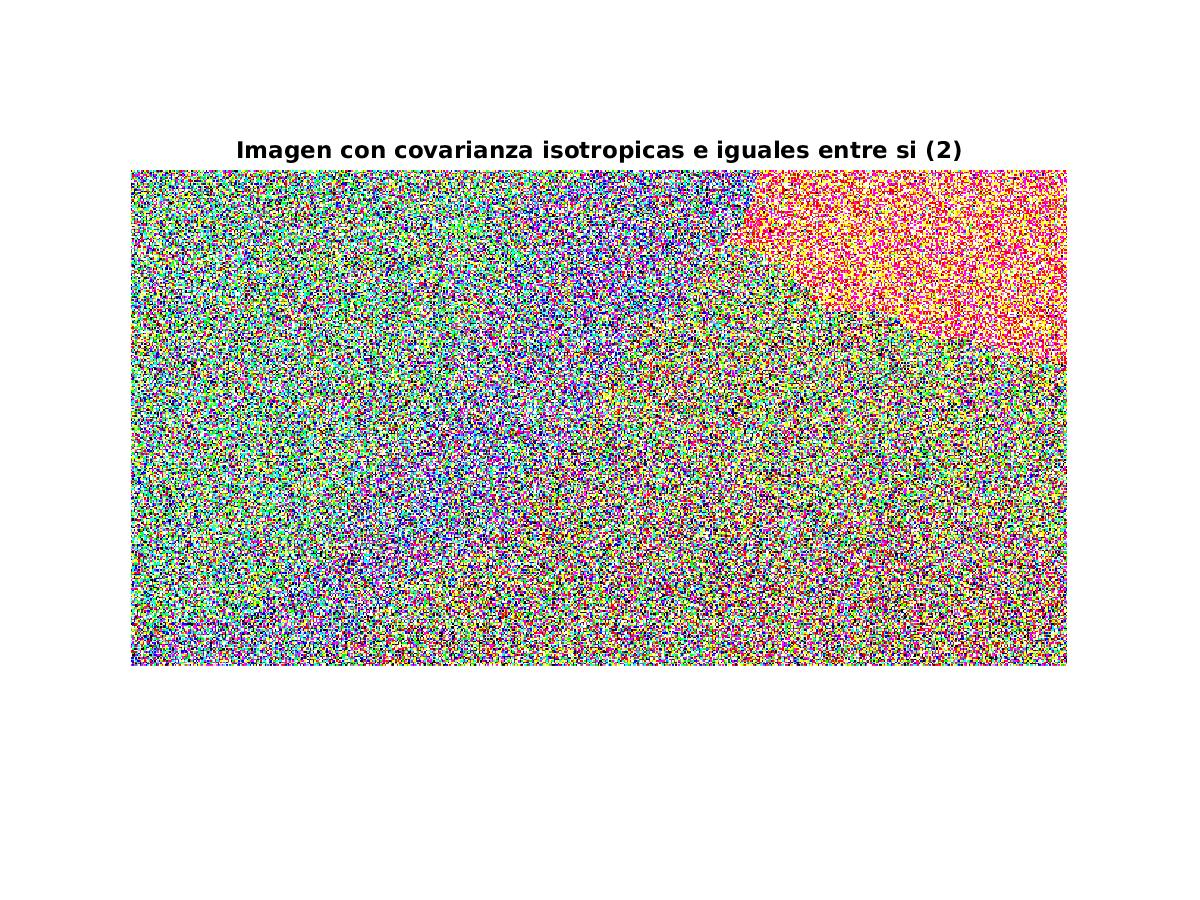
\includegraphics[width=90mm]{imagenII2.jpg}
\caption{Usando sigma2}
\end{figure}


Y estas son sus tablas de comfuci\'on:

Tabla de confusi\'on del caso con covarianza isotr\'opicas e iguales entre si. (sigma1)\newline
\begin{tabular}{| l | l | l | l | l | l | l | }
      & Caso1 & Caso2 & Caso3 & Caso4 & Caso5 & Caso6\\ \hline
Caso1 &       42180     &   7460         &  0  &      6948      &  5057 &        643\\ \hline
Caso2 &        4295     &  31570        &   0   &      277     &   2068  &      1049\\ \hline
Caso3 &           0      &     0       &22325    &       0    &       0   &        1\\ \hline
Caso4 &        5356       & 1089       &    0     &  18286   &     6118    &    7686\\ \hline
Caso5 &        4127       & 2830      &     0      &  8123  &      9113     &   9297\\ \hline
Caso6 &         493        & 913     &      0       & 3476 &       3244      & 11620\\ \hline
\end{tabular}\newline

Tabla de confusi\'on del caso con covarianza isotr\'opicas e iguales entre si. (sigma2)\newline
\begin{tabular}{| l | l | l | l | l | l | l | }
      & Caso1 & Caso2 & Caso3 & Caso4 & Caso5 & Caso6\\ \hline
Caso1 &       18294   &    17620      &  9919 &       7852      &  1806 &       6797\\ \hline
Caso2 &        8800    &   14855     &   6613  &      3392     &   1086  &      4513\\ \hline
Caso3 &         899     &   1929    &   15937   &     1537    &     106   &     1918\\ \hline
Caso4 &        8959      &  8967   &     8399    &    5696   &     1165    &    5349\\ \hline
Caso5 &        7353       & 8972  &      6968     &   4250  &      1015     &   4932\\ \hline
Caso6 &        3759        &4872 &       4861      &  2527 &        581      &  3146\\ \hline
\end{tabular}


\subsection{Utilizando matrices de covarianza diagonales y diferentes para cada clase}

Se toma las siguientes matrices de covarianza:

sigma1 = 
\begin{tabular}{ l c r }
  0.5 & 0 & 0 \\
  0 & 0.4 & 0 \\
  0 & 0 & 0.7 \\
\end{tabular}


sigma2 =
\begin{tabular}{ l c r }
  89.8 & 0 & 0 \\
  0 & 37 & 0 \\
  0 & 0 & 54.2 \\
\end{tabular}


Con estas se generaron las siguientes im\'agenes:

\begin{figure}[H]
\centering
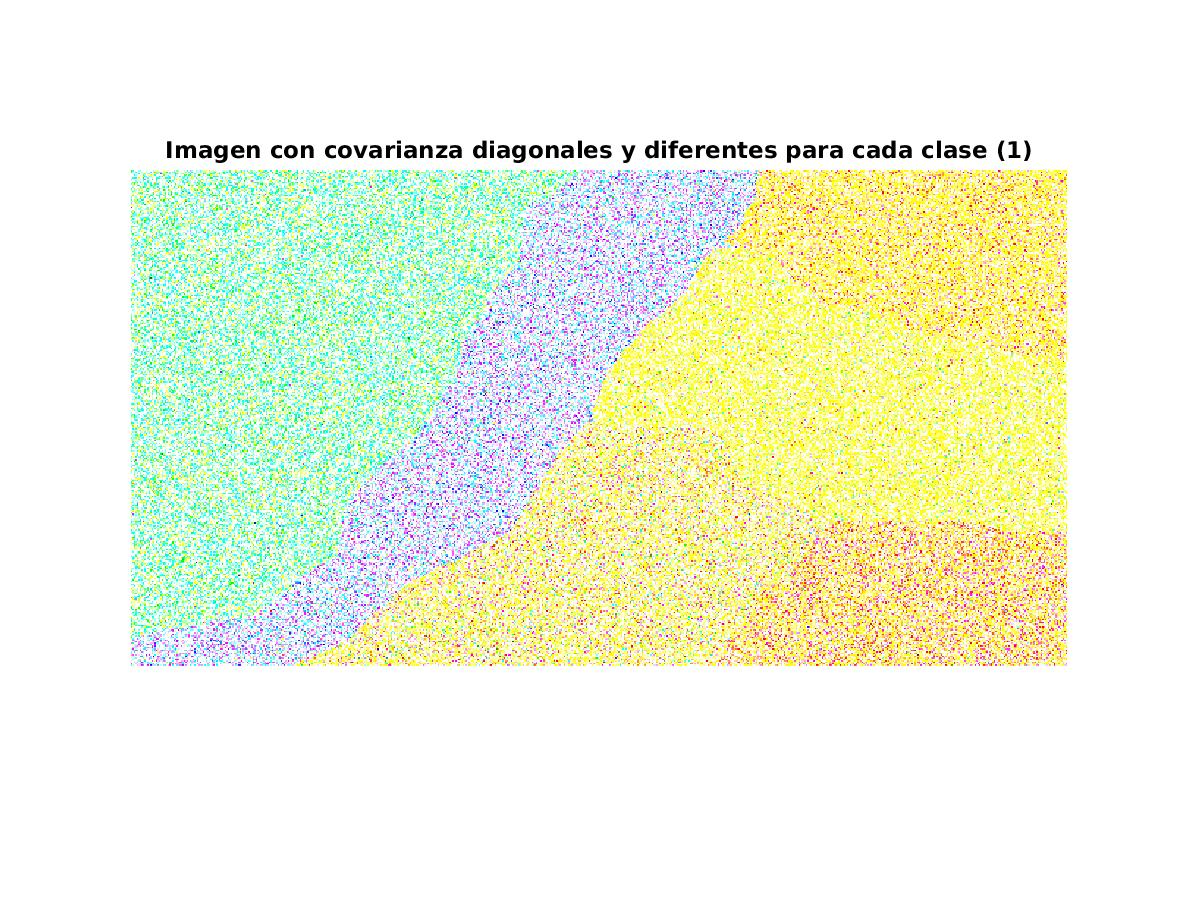
\includegraphics[width=90mm]{imagenDD1.jpg}
\caption{Usango sigma1}
\end{figure}


\begin{figure}[H]
\centering
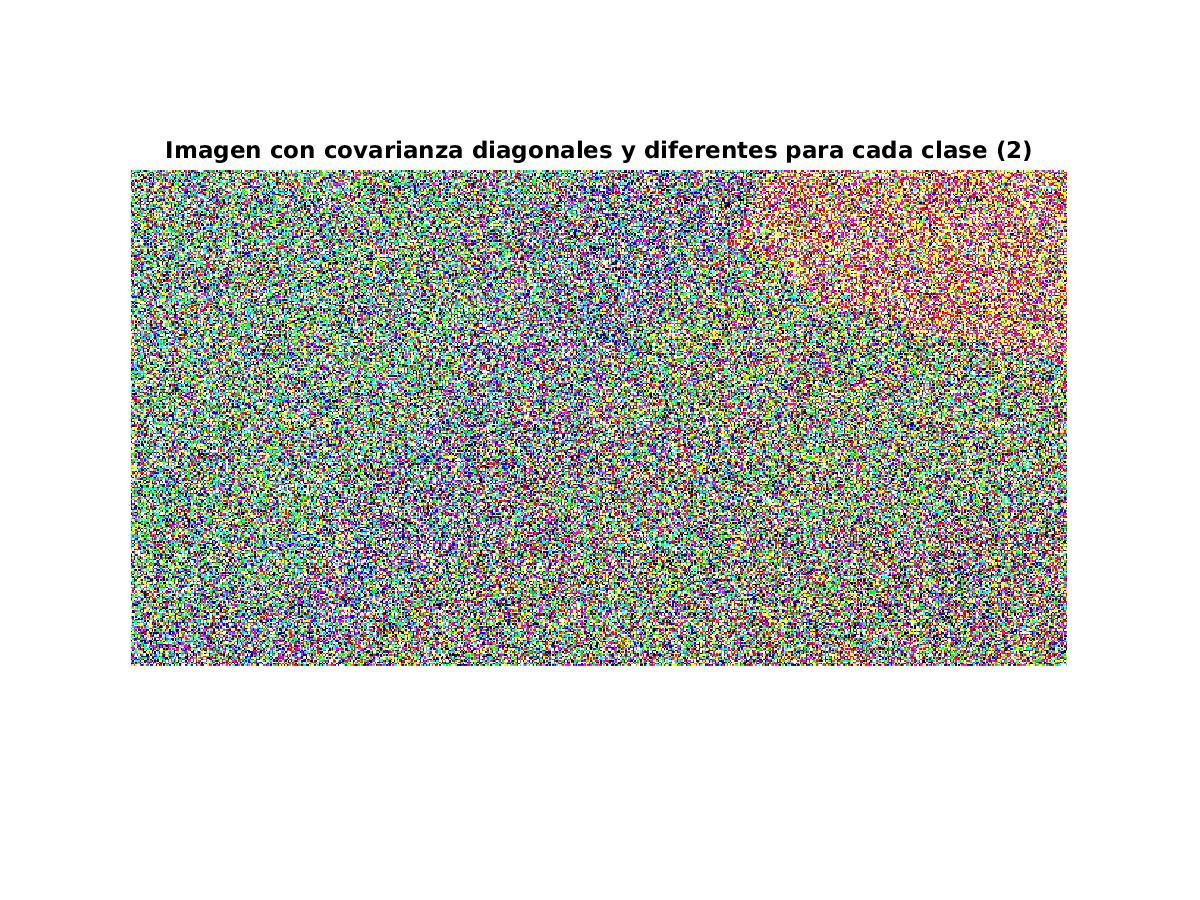
\includegraphics[width=90mm]{imagenDD2.jpg}
\caption{Usando sigma2}
\end{figure}


Y estas son sus tablas de comfusi\'on:

Tabla de confusi\'on del caso con covarianza diagonales y diferentes para cada clase. (sigma1)\newline
\begin{tabular}{| l | l | l | l | l | l | l | }
& Caso1 & Caso2 & Caso3 & Caso4 & Caso5 & Caso6\\ \hline
Caso1 &       42612       & 7228      &     0&        7601     &   4294&         553\\ \hline
Caso2 &        4311       &30110     &      0 &        544    &    2681 &       1613\\ \hline
Caso3 &           0        &   0    &   22326  &         0   &        0  &         0\\ \hline
Caso4 &        5700        &1460   &        0   &    18495  &      5869   &     7011\\ \hline
Caso5 &        3755        &3677  &         0    &    8106 &       8726    &    9226\\ \hline
Caso6 &         428        &1214 &          0     &   3189&        3075     &  11840\\ \hline


\end{tabular}\newline

Tabla de confusi\'on del caso con covarianza diagonales y diferentes para cada clase. (sigma2)\newline
\begin{tabular}{| l | l | l | l | l | l | l | }
& Caso1 & Caso2 & Caso3 & Caso4 & Caso5 & Caso6\\ \hline
Caso1 &       16468       &16363       &17221        &5513        &1261        &5462\\ \hline
Caso2 &        8620       &12546       &10980        &2665         &734        &3714\\ \hline
Caso3 &        2654        &3602       &12467        &1569         &226        &1808\\ \hline
Caso4 &        8948        &9090       &12170        &3656         &795        &3876\\ \hline
Caso5 &        7365        &8467       &10486        &3028         &681        &3463\\ \hline
Caso6 &        3984       & 4860        &6476        &1772         &422        &2232\\ \hline
\end{tabular}

\subsection{Utilizando matrices de covarianza no diagonales y diferentes para cada clase}

Se toma las siguientes matrices de covarianza:


sigma1 = 
\begin{tabular}{ l c r }
  0.6 & 0.3 & 0.2 \\
  0.3 & 0.2 & 0.15 \\
  0.2 & 0.15 & 0.12 \\
\end{tabular}


sigma2 =
\begin{tabular}{ l c r }
  12 & 6 & 4 \\
  6 & 4 & 3 \\
  4 & 3 & 2.4 \\
\end{tabular}

Con estas se generaron las siguientes im\'agenes:

\begin{figure}[H]
\centering
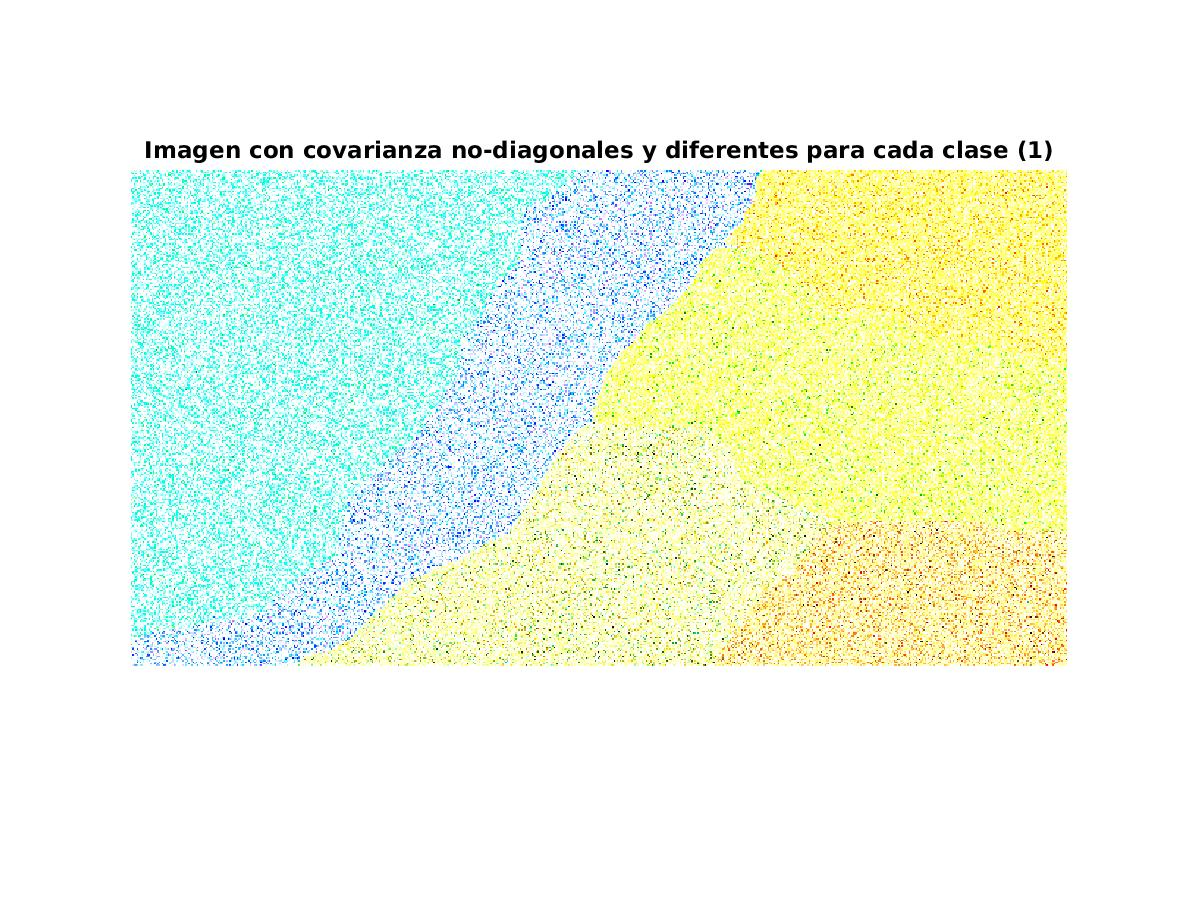
\includegraphics[width=90mm]{imagennDD1.jpg}
\caption{Usango sigma1}
\end{figure}


\begin{figure}[H]
\centering
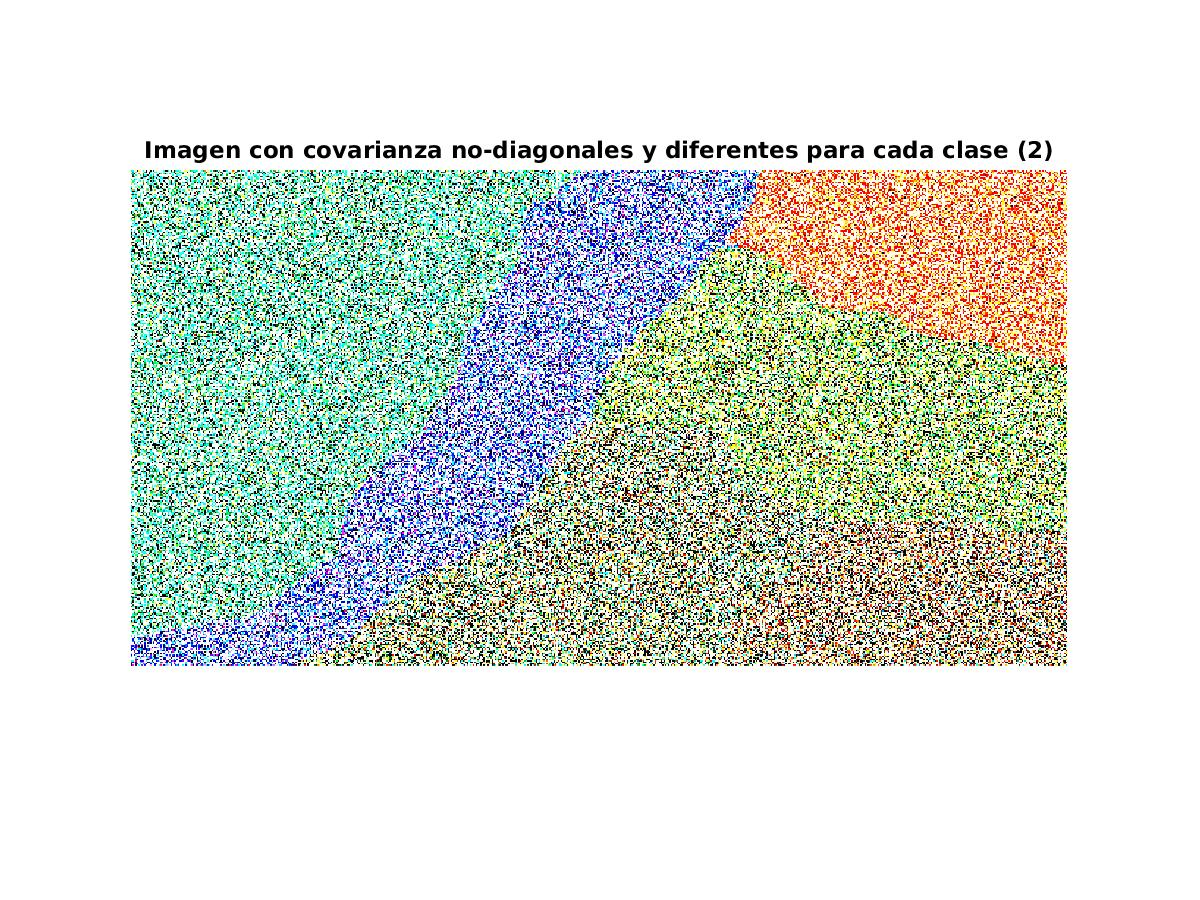
\includegraphics[width=90mm]{imagennDD2.jpg}
\caption{Usando sigma2}
\end{figure}

Y estas son sus tablas de comfusi\'on:

Tabla de confusi\'on del caso con covarianza no diagonales y diferentes para cada clase. (sigma1)\newline

\begin{tabular}{| l | l | l | l | l | l | l |} 
& Caso1 & Caso2 & Caso3 & Caso4 & Caso5 & Caso6\\ \hline
Caso1 &     62218&           0      &     0 &         70      &     0&           0\\ \hline
Caso2 &           0 &      39259     &      0  &         0     &      0 &          0\\ \hline
Caso3 &           0  &         0    &   22326   &        0    &       0  &         0\\ \hline
Caso4 &          63   &        0   &        0    &   38472   &        0   &        0\\ \hline
Caso5 &           0    &       0  &         0     &      0  &     33144    &     346\\ \hline
Caso6 &           0     &      0 &          0      &     0 &        214     &  19532\\ \hline
\end{tabular}\newline

Tabla de confusi\'on del caso con covarianza no diagonales y diferentes para cada clase. (sigma2)\newline

\begin{tabular}{| l | l | l | l | l | l | l | }
& Caso1 & Caso2 & Caso3 & Caso4 & Caso5 & Caso6\\ \hline
Caso1 &	37892&           0     &      1&       14966    &    9024&         405\\ \hline
Caso2 &           0  &     39074     &    146  &         0    &       0  &        39\\ \hline
Caso3 &           0   &       83    &   21555   &        0   &        0   &      688\\ \hline
Caso4 &        8212    &       0   &        0    &   27890  &      2348    &      85\\ \hline
Caso5 &        4302     &      5  &        90     &   1888 &      17296     &   9909\\ \hline
Caso6 &         327      &    23 &        589      &   181&        5463      & 13163\\ \hline

\end{tabular}

\subsection{Conclusiones}
Como podemos ver si hacemos m\'as grandes los valores de la matriz de covarianza la imagen generada se ve menos n\'itida y se vuelve mas dif\'icil a simple vista distinguir los colores. Esto tambi\'en se traduce en la tabla de confusi\'on donde entre mas varianza haya la misma dispersara mas los valores. Esto provoca que al verla como matriz esta sea, por decirlo de alguna manera, menos diagonalmente dominante.


\section{Ejercicio 2}
Para \'este punto tenemos que extraer datos de las regiones de entrenamiento y calcular su valor medio y covarianza.

\begin{figure}[H]
\centering
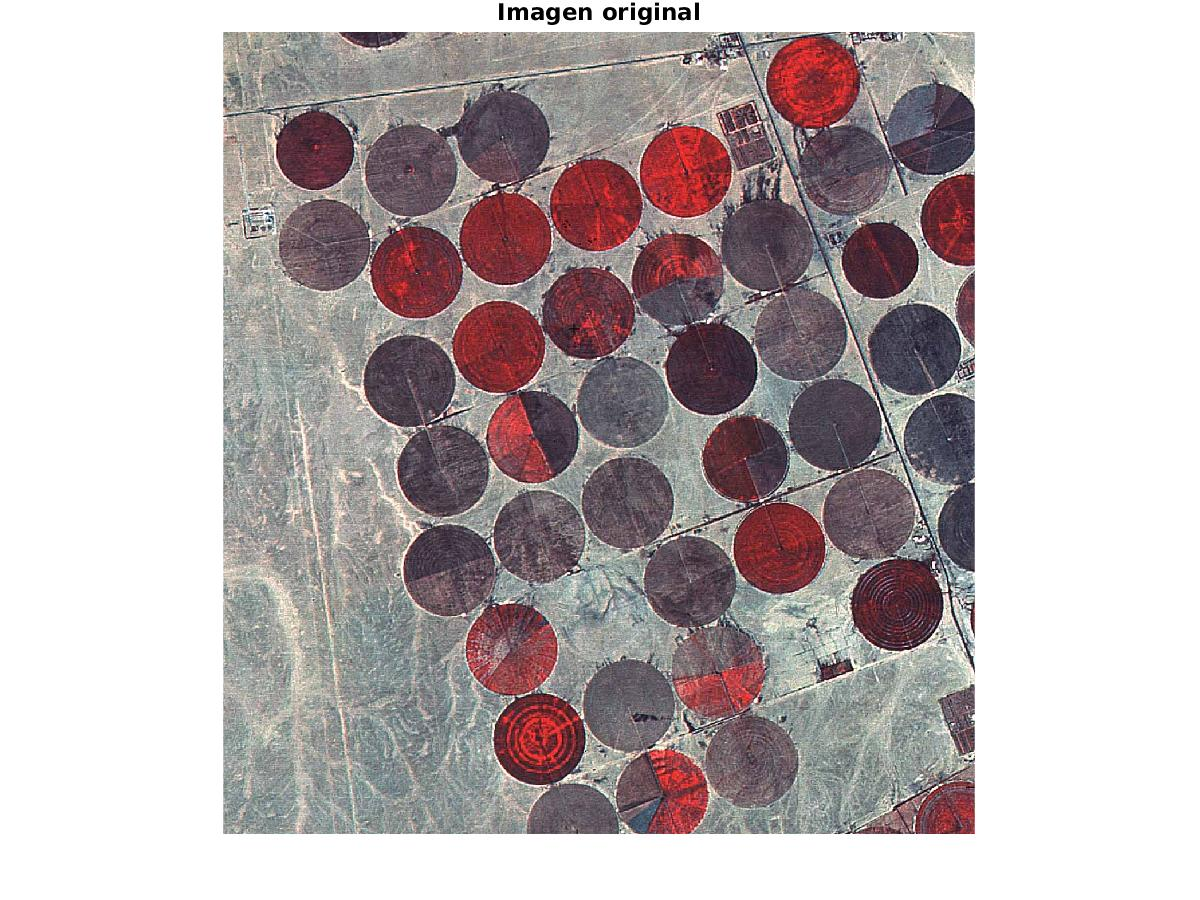
\includegraphics[width=90mm]{ImagenNormal.jpg}
\caption{Esta es la imagen normal}
\end{figure}

\begin{figure}[H]
\centering
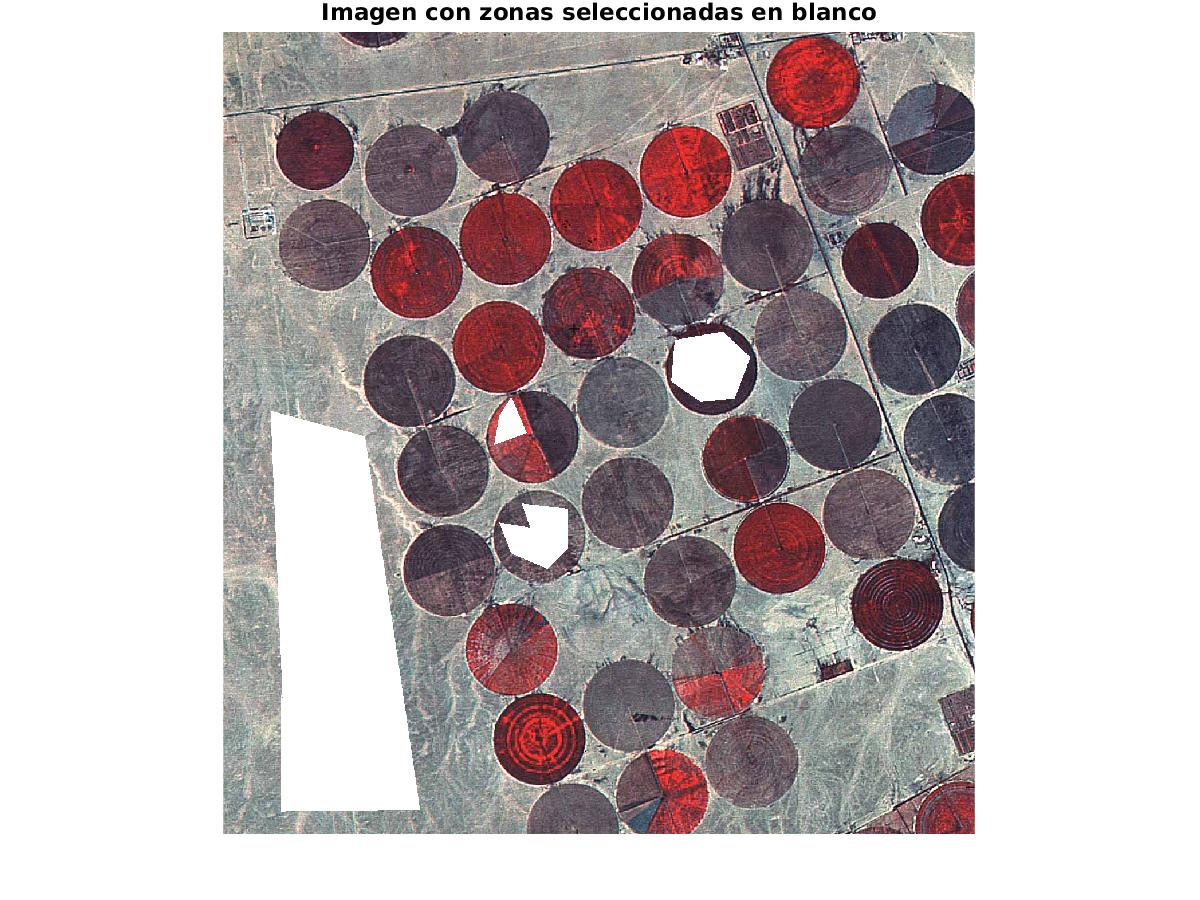
\includegraphics[width=90mm]{imagenBlanco.jpg}
\caption{Esta es la imagen con las regiones de entrenamiento marcadas}
\end{figure}

\begin{figure}[H]
\centering
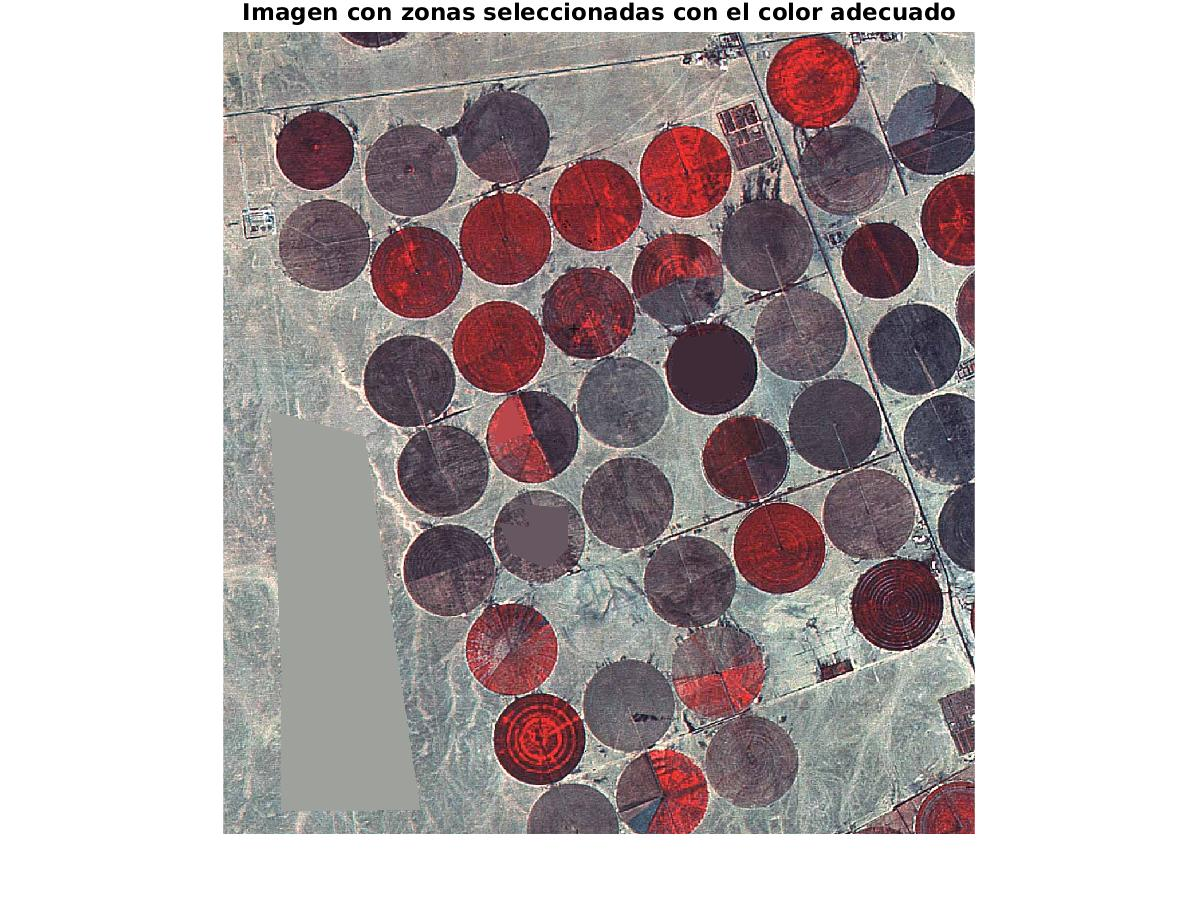
\includegraphics[width=90mm]{imagenColores.jpg}
\caption{Esta es la imagen con las regiones de entrenamiento marcadas y coloreadas para diferenciarlas}
\end{figure}

Valor medio para la zona gris= $(159.1992 , 160.9931 , 156.2931)$\\

Valor medio para la zona gris oscuro= $(101.7899 , 87.4822 , 95.7200)$\\

Valor medio para la zona negra= $(63.4611 , 41.5487 , 54.7426)$\\

Valor medio para la zona roja= $(184.9976 , 71.3169 , 75.95761)$\\

Covarianza para zona gris =
\begin{tabular}{ l c r }
  946.5474 & 752.1900 & 659.5253\\
  752.1900  &677.9327 & 599.7840\\
  659.5253  &599.7840 & 557.4782\\
\end{tabular}\newline

Covarianza para zona gris oscuro=
\begin{tabular}{ l c r }
  590.0180&  562.2911  &529.4815\\
  562.2911 & 579.7685 & 536.8973\\
  529.4815  &536.8973&  512.0039\\
\end{tabular}\newline

Covarianza para zona negra=
\begin{tabular}{ l c r }
  102.4073&   71.1859  & 71.7668\\
   71.1859 &  74.0204 &  72.9073\\
   71.7668  & 72.9073&   77.0635\\
\end{tabular}\newline

Covarianza para zona roja=
\begin{tabular}{ l c r }
  852.1874&  157.6038  &173.0104\\
  157.6038 & 165.8111 & 160.8769\\
  173.0104  &160.8769&  192.0786\\
\end{tabular}\newline

Lo siguiente que pide el enunciado es clasificar la imagen. Para esto calculare la covarianza de la imagen que tendr\'a el nombre sigma. 

Los valores medio para clasificar ser\'an los calculados anteriormente.
Una vez clasificada la imagen, se debe hacer lo mismo con cada una de las regiones de entrenamiento y calcular la tabla de confusi\'on para cada uno de los casos.\newline


Tabla de confusión zona gris:\newline

\begin{tabular}{ | l | l | l | l | l |  }
		& Gris &   Gris Oscuro     & Rojo    & Negro\\ \hline
  Gris    	&       122525       & 1752  &         0&           0\\ \hline
  Gris Oscuro   &      8452       & 1240    &       0    &       0\\ \hline
  Rojo       	&         11       &   65  &         0    &       0\\ \hline
  Negro       	&         35        &  19 &          0     &      2\\ \hline
 
\end{tabular}\newline


Tabla de confusión zona gris oscuro:\newline

\begin{tabular}{ | l | l | l | l | l |  }
		& Gris &   Gris Oscuro     & Rojo    & Negro\\ \hline
Gris &	  	249 &        212  & 0 &       0\\ \hline
Gris Oscuro &    93   &     6059  &   0 &   358\\ \hline
Rojo		 & 0 & 0& 0 & 0\\ \hline
Negro &           1    &    1093 &   0   &  939\\ \hline
\end{tabular}\newline

Tabla de confusión zona negra:\newline

\begin{tabular}{ | l | l | l | l | l |  }
		& Gris &   Gris Oscuro     & Rojo    & Negro\\ \hline
Gris          & 0   &        0  &   0&      0\\ \hline
Gris Oscuro          & 5  &        49   &  0&    330\\ \hline
Rojo & 0  &  0  &  0 & 0\\ \hline
Negro          & 0 &         12  & 0 &   12366\\ \hline

\end{tabular}\newline

Tabla de confusión zona roja:\newline

\begin{tabular}{| l | l | l | l | l |  }
		& Gris &   Gris Oscuro     & Rojo    & Negro\\ \hline
Gris          & 0    &       0   &        5     &      0\\ \hline
Gris Oscuro          & 0   &       34    &      65    &      11\\ \hline
Rojo          & 0  &        32     &   2321   &        1\\ \hline
Negro          & 0 &          0      &     4  &         4\\ \hline
\end{tabular}\newline
           
Por \'ultimo se debe repetir el proceso anterior pero seleccionando zonas de entrenamiento propias. Para resolver este problema se llego la decisi\'on de tomar una serie de puntos de cada una de las zonas de entrenamiento anteriores, osea una parte de la zona, y calcular la tabla de confusi\'on utilizando esa parte. De esta forma se cumple el enunciado y adem\'as se ahorra el clasificar nuevamente una zona que ya lo est\'a. \newline


Tabla de confusión zona gris propia:\newline
\begin{tabular}{ | l | l | l | l | l |  }
		& Gris &   Gris Oscuro     & Rojo    & Negro\\ \hline
  Gris &             3709  &        46 & 0 & 0\\ \hline
    Gris Oscuro &       177        &  68 & 0 & 0\\ \hline

  Rojo  &   0 & 0 & 0 & 0\\ \hline
  Negro & 0 & 0 & 0 & 0\\ \hline
\end{tabular}\newline

Tabla de confusión zona gris oscuro propia:\newline
\begin{tabular}{| l | l | l | l | l |  }
		& Gris &   Gris Oscuro     & Rojo    & Negro\\ \hline
Gris		&15   &       44  &  0   &    0\\ \hline
Gris Oscuro		&20  &      2766   & 0  &   123\\ \hline
Rojo		&0   &   0   &  0  & 0\\ \hline
Negro		&0  &       536     &0 &   496\\ \hline
\end{tabular}\newline

Tabla de confusión zona negra propia:\newline
\begin{tabular}{| l | l | l | l | l | }
		& Gris &   Gris Oscuro     & Rojo    & Negro\\ \hline
Gris         &  0    &       0  & 0 &         0\\ \hline
Gris Oscuro &          1      &    10    & 0  &     116\\ \hline
Rojo  &  0  &  0 & 0  & 0\\ \hline
Negro   &        0         &  0    &0 &    3873\\ \hline
\end{tabular}\newline

Tabla de confusión zona roja propia:\newline
\begin{tabular}{| l | l | l | l | l | }
		& Gris &   Gris Oscuro     & Rojo    & Negro\\ \hline
Gris     &0    & 0&     5    & 0\\ \hline
Gris Oscuro     &0   & 31 &   44   & 10\\ \hline
Rojo     &0  &  29  & 880  &   1\\ \hline
Negro     &0 &    0   &  0 &    0\\ \hline
\end{tabular} 

\subsection{Conclusiones}

Como podemos ver tanto en el caso de las regiones de entrenamiento, tanto provistas como las propias, tenemos que cada una de las matrices tienen como mayor numero de coincidencias a los colores de sus respectivas zonas. O lo que es lo mismo, la clasificaci\'on muestra que en la zona de un color lo que predomina es ese color por sobre los dem\'as.

\end{document}